\documentclass[a4paper, 12pt]{article}
\usepackage{polski}
\usepackage[font=scriptsize]{caption}
\usepackage{indentfirst}
\usepackage{amsmath}
\usepackage{amssymb}
\usepackage{graphicx}
\usepackage{longtable}
\usepackage{color, colortbl}
\usepackage[title]{appendix}
\usepackage{hyperref}
\usepackage{tabularx}
\usepackage[polish]{babel}

\newcommand{\nl}{\\\hline}

\begin{document}
\title{
    \huge{Sieci złożone} \\
    \small{Sprawozdanie}
}
\author{Przemysław Barcicki}
\maketitle

\thispagestyle{empty}

\section{Wstęp}
Celem mojego zadania było zebranie danych na temat pewnej sieci złożonej oraz zbadanie jej pod względem różnych właściwości ze świata teorii grafów. Różnych sieci które charakteryzują się tą złożonością, jest wiele, przykładowo są to sieci współpracy, znajomości, kontaktów seksualnych czy nawet Internet.

Do swoich badań wybrałem połączenia między artykułami na internetowej encyklopedii Wikipedia, gdzie, wierzchołkami w grafie są różne artykuły, a krawędziami (jednokieurnkowymi) są odnośniki i nawiązania między artykułami. Dzięki historii zmian przypisanej do każdej podstrony można dodatkowo zbadać artykuł pod względem rozwoju danej dziedziny, czy też rozwoju samego artykułu, w domenie czasowej. Aby nie dochodziło do dużego wybuchu ilości odnośników w swoich badaniach ograniczyłem się tylko do jednej konkretnej kategorii (artykuł \textit{Informatyka} ma 535 odnośników do innych artykułów z czego tylko 9 dotyczy surowej kategorii Informatyka\footnote{Stan na 03.01.2023}). Analizę będę przedstawiał na zbiorze danych z polskiej kategorii informatyka.

\section{Zbieranie danych}
Zbieranie danych bazowało na wysyłaniu zapytań do ogólnodostępnego interfejsu programowego wikipedii, gdzie odpowiednio dobierając argumenty można było pytać o konkretne zasoby zawarte na stronie, bez ściągania jej całej, razem z odpowiednim filtrowaniem danych. Tak jak wspomniałem wcześniej, dane filtrowane były na podstawie kategorii. W grafach wyjściowych znajdują się wszystkie artykuły z kategorii oraz dodatkowo artykuł znajdujący się na obrzeżach, który jako pierwszy wychodzi z danej kategorii (najczęściej będą to wierzchołki ze stopniem 1).

\section{Analiza danych}
Najprostszym elementem do analizy jest przegląd jak zmieniała się wielkość kategorii w czasie. Wykres (\ref{fig:size_pl}) obrazuje tą zmianę w czasie.
\begin{center}
    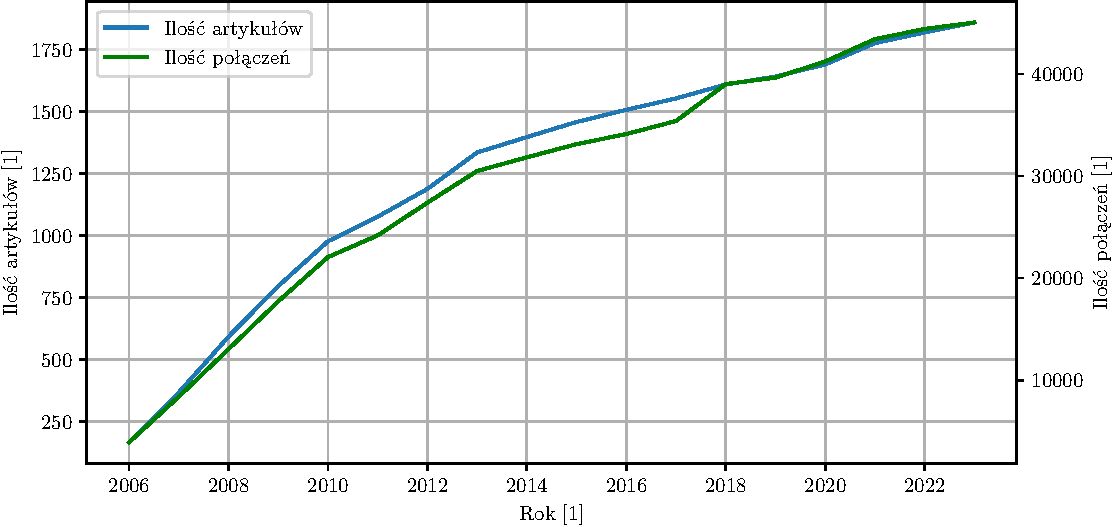
\includegraphics[width=0.90\linewidth]{figures/size_pl.pdf}
    \label{fig:size_pl}
    \captionof{figure}{Wykres przedstawiający wielkość kategorii Informatyka w czasie. Niebieskim kolorem przedstawiono artykuły, zielonym ilość połączeń między artykułami.}
\end{center}
Można zauważyć, że ilość połączeń między akrtykułami jest powiązana liniowo z liczbą artykułów, sugeruje to że, artykuły dodawane do kategorii, nie nawiązują do dużej ilości innych artykułów w tej samej kategorii.

Kolejno można przedstawić, jak zmieniała się gęstość grafu na przestrzeni czasu. Sama wielkość opisuje stosunek między ilością połączeń w grafie a ilością możliwych połączeń.
\begin{center}
    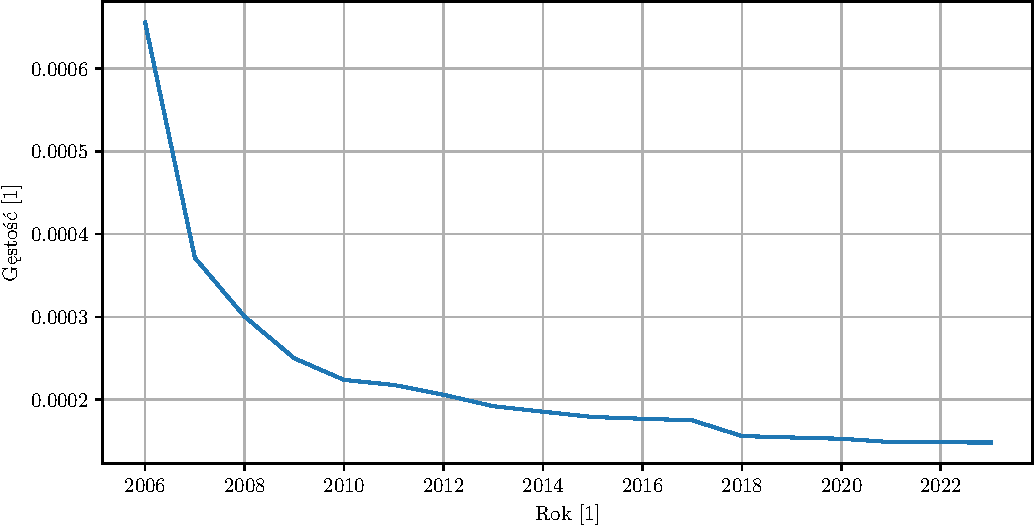
\includegraphics[width=0.90\linewidth]{figures/density_pl.pdf}
    \captionof{figure}{Wykres przedstawiający gęstość grafu opisującego kategorię Informatyka w czasie.}
    \label{fig:denisty_pl}
\end{center}
Na wykresie (\ref{fig:denisty_pl}) widać, że wraz z rozwojem informatyki na przestrzeni ostatnich 15 lat, graf się rozrzadził. Jest to logiczne, wraz z powstawaniem nowych podkategorii, zasięg informatyki zwiększa się, lecz niekoniecznie są one mocno powiązane z istniejącymi już kategoriami.

Aby zbadać średnią długość (najkrótszej) ścieżki musimy skorzystać z pewnych uproszczeń, w których dla każdego grafu wybieramy największy słabo spójny komponent. Tym procesem nie tracimy dużo informacji z wykluczonych wierzchołków, ponieważ w każdym roku, wielkość największego komponentu stanowi przynajmniej 99.5\% wielkości całego grafu.

\begin{center}
    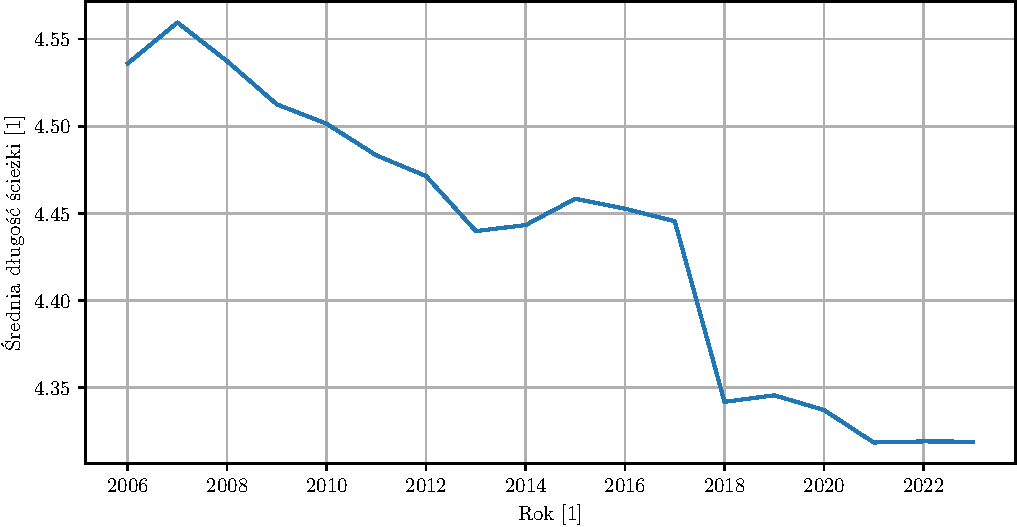
\includegraphics[width=0.90\linewidth]{figures/path_pl.pdf}
    \captionof{figure}{Wykres przedstawiający średnią długość najkrótszych ścieżek między wierzchołkami.}
    \label{fig:path_pl}
\end{center}
Spadająca wartość średniej długości ścieżki na wykresie (\ref{fig:path_pl}) może sugerować konsolidację poprzez powstanie tematów, kategorii czy artykułów które spinają ze sobą dalsze witryny, ale także, co widać po wykresie ilości wszystkich połączeń, że istniejące już tematy, zostały uzupełnione o odpowiednie odnośniki do istniejących wierzchołków.
\newpage

Kolejną istotną charakterystyką sieci połączeń jest rozkład stopni wierzchołków. Wielkość ta, może nam sugerować jak dobrze połączone są ze sobą konkretne tematy w konkretnej kategorii. Histogram tego rozkładu przedstawia rysunek (\ref{fig:degreehist_pl}), a tabela (\ref{tab:maxmean_pl}) zawiera informację o maksymalnym i średnim wierzchołku.

\begin{center}
    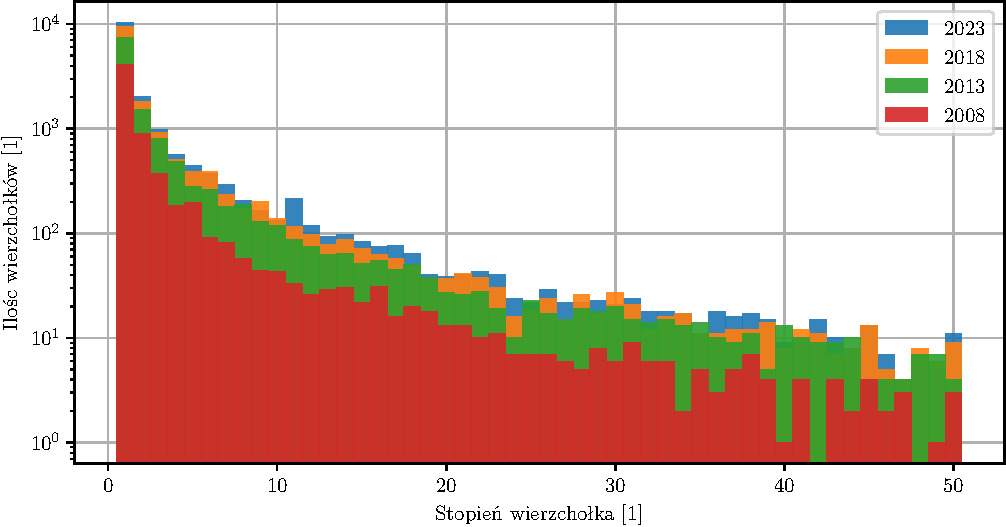
\includegraphics[width=0.90\linewidth]{figures/degreehist_pl.pdf}
    \captionof{figure}{Wykres przedstawiający rozkład stopni wierzchołków w grafie dla różnych lat.}
    \label{fig:degreehist_pl}
\end{center}
\begin{center}
    \captionof{table}{Tabela przedstawiająca zmianę maksymalnej i średniej wartości stopnia wierzchołka na przestrzeni lat.}
    \begin{tabular}{|c|c|c|c|}
	\hline
	Rok &	Max &	Średnia &	Artykuł \nl
	2008 &	301 &	3.943 &	Pulpit \nl
	2011 &	311 &	4.551 &	Język angielski \nl
	2014 &	390 &	4.81 &	Język angielski \nl
	2017 &	423 &	4.931 &	Język angielski \nl
	2020 &	847 &	4.972 &	Skróty używane w informatyce \nl
	2023 &	847 &	5.115 &	Skróty używane w informatyce \nl
\end{tabular}
    \label{tab:maxmean_pl}
\end{center}

Pewną dodatkową charakterystyką opisującą ważność danego wierzchołka jest jak wiele najkrótszych ścieżek przechodzi przez dany element w grafie, ta charakterystyka opisuje nam pewien najważniejszy centraly przegub którego usunięcie zmieniłoby strukturę całej sieci. W tabeli (\ref{tab:joints_pl}) zawarto informację o ilości ścieżek przechodzących przez jaki wierzchołek.

\newpage

\begin{center}
    \captionof{table}{Tabela przedstawiająca wierzchołki z największą ilością ścieżek na przestrzeni lat.}
    \begin{tabular}{|c|c|c|}
	\hline
	Rok &	Artykuł &	Ścieżki \nl
	2008 &	Moc obliczeniowa &	6.12\% \nl
	2011 &	Program komputerowy &	2.8\% \nl
	2014 &	Program komputerowy &	2.08\% \nl
	2017 &	Program komputerowy &	1.71\% \nl
	2020 &	Informatyka &	2.78\% \nl
	2023 &	Informatyka &	2.6\% \nl
\end{tabular}
    \label{tab:joints_pl}
\end{center}

\section{Wnioski}
Na przedstawionych wykresach, widać rozwój kategorii Informatyka, razem z rozwojem samej Wikipedii. Wraz z czasem pojawiło się tam kilkukrotnie więcej artykułów i połączeń między nimi, co można powiązać w dużej mierze z rozwojem informatyki, ale także większą dostępnością internetu dla ludzi w całym kraju. Im więcej ludzi z niej korzysta, tym więcej osób się znajdzie, którzy (za darmo) poświęcą swój czas i wiedzę dla rozwoju ogółu.

\begin{appendices}

\section{Angoljęzyczne porównanie}
Poniższe rysunki (\ref{fig:size_en}, \ref{fig:density_en}, \ref{fig:path_en}, \ref{fig:degreehist_en}) oraz tabele (\ref{tab:joints_en}, \ref{tab:maxmean_en}) przedstawiają porównanie polskiej oraz anglojęzycznej wersji kategorii Informatyka na stronie Wikipedia.

\begin{center}
    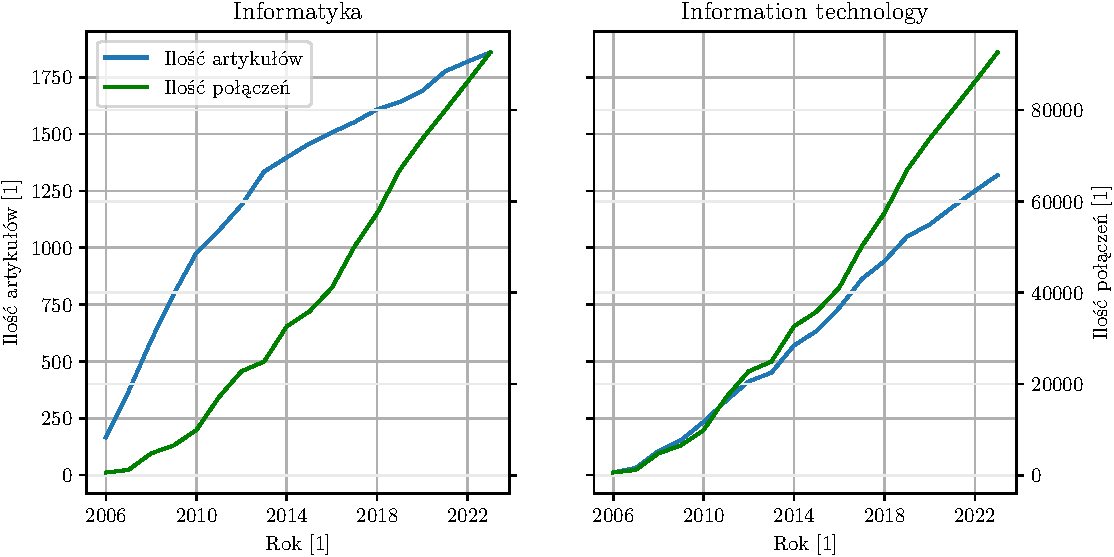
\includegraphics[width=\linewidth]{figures/size_en.pdf}
    \captionof{figure}{Wykres przedstawiający wielkość kategorii Informatyka w czasie. Niebieskim kolorem przedstawiono artykuły, zielonym ilość połączeń między artykułami.}
    \label{fig:size_en}
\end{center}

\begin{center}
    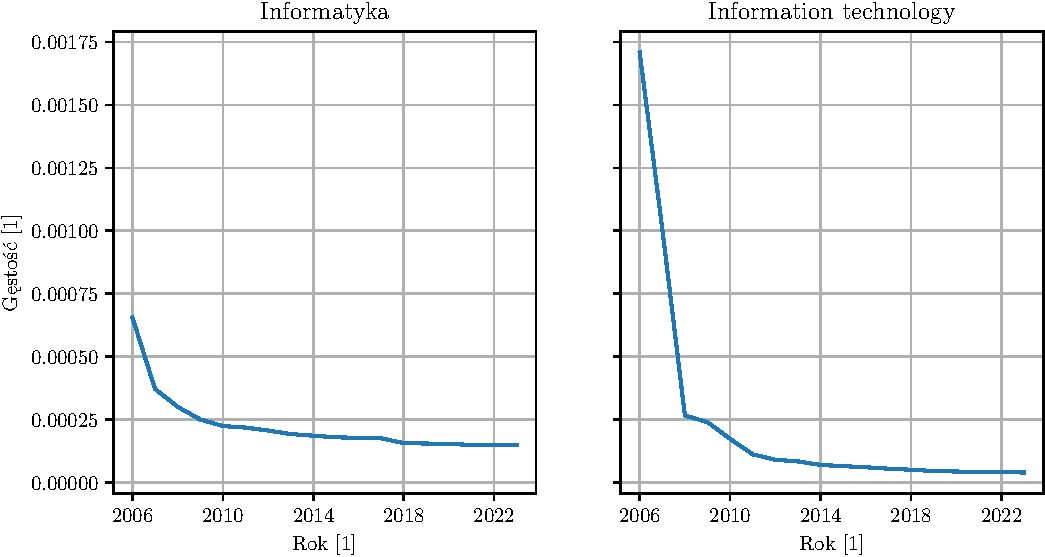
\includegraphics[width=\linewidth]{figures/density_en.pdf}
    \captionof{figure}{Wykres przedstawiający gęstość grafu opisującego kategorię Informatyka w czasie.}
    \label{fig:density_en}
\end{center}

\begin{center}
    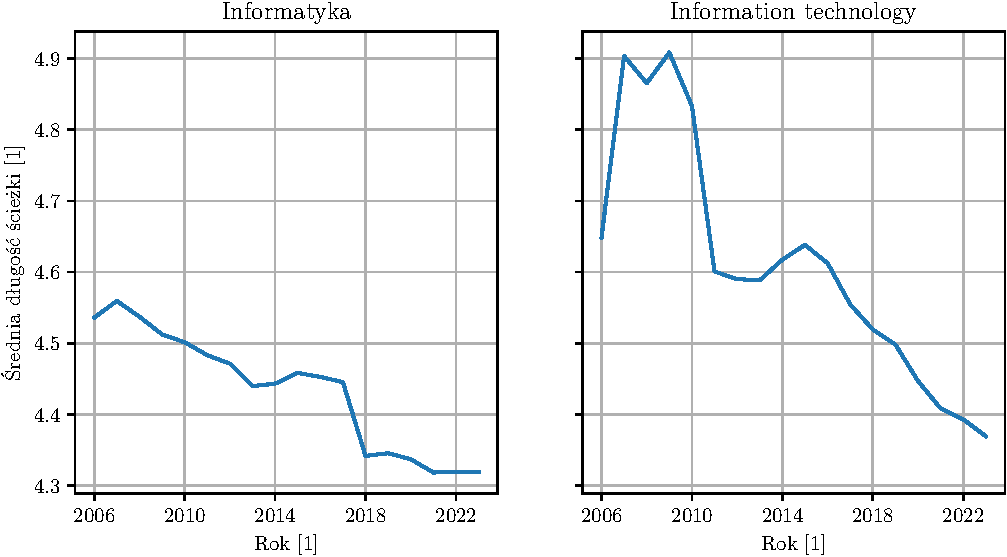
\includegraphics[width=\linewidth]{figures/path_en.pdf}
    \captionof{figure}{Wykres przedstawiający średnią długość najkrótszych ścieżek między wierzchołkami.}
    \label{fig:path_en}
\end{center}

\begin{center}
    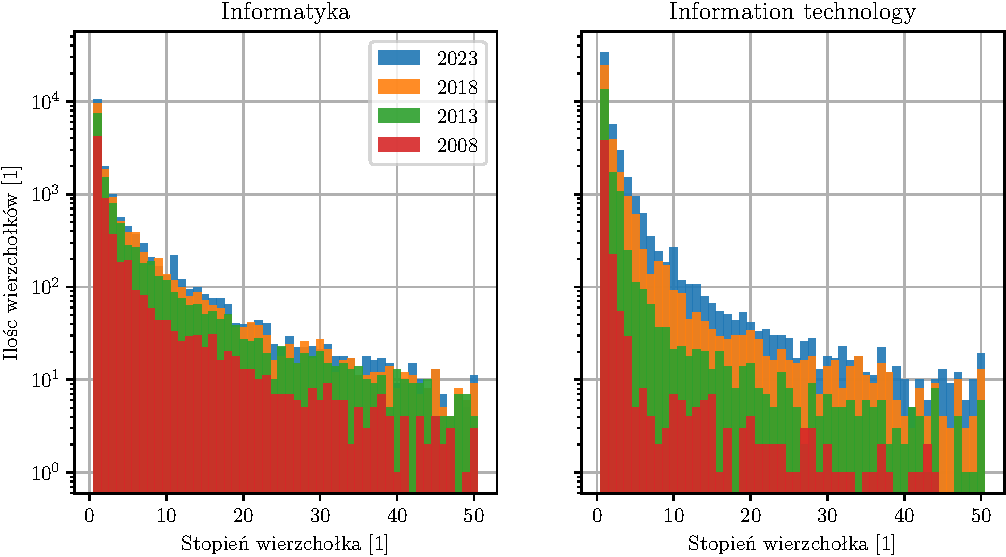
\includegraphics[width=\linewidth]{figures/degreehist_en.pdf}
    \captionof{figure}{Wykres przedstawiający rozkład stopni wierzchołków w grafie dla różnych lat.}
    \label{fig:degreehist_en}
\end{center}

\begin{center}
    \captionof{table}{Tabela przedstawiająca zmianę maksymalnej i średniej wartości stopnia wierzchołka na przestrzeni lat.}
    \begin{tabular}{|c|c|c|c|}
	\hline
	Rok &	Max &	Średnia &	Artykuł \nl
	2008 &	626 &	2.255 &	Information industry \nl
	2011 &	626 &	2.761 &	Information industry \nl
	2014 &	627 &	3.003 &	Information industry \nl
	2017 &	741 &	3.29 &	Linus Torvalds \nl
	2020 &	899 &	3.534 &	Digital media use and mental health \nl
	2023 &	998 &	3.781 &	Silicon Valley \nl
\end{tabular}
    \label{tab:maxmean_en}
\end{center}

\begin{center}
    \captionof{table}{Tabela przedstawiająca wierzchołki z największą ilością ścieżek na przestrzeni lat.}
    \begin{tabular}{|c|c|c|}
	\hline
	Rok &	Artykuł &	Ścieżki \nl
	2008 &	Information industry &	5.75\% \nl
	2011 &	Real-time business intelligence &	1.94\% \nl
	2014 &	Information society &	6.85\% \nl
	2017 &	Metadata &	7.85\% \nl
	2020 &	Business intelligence &	4.52\% \nl
	2023 &	Information technology &	3.16\% \nl
\end{tabular}
    \label{tab:joints_en}
\end{center}

\newpage

\section{Kod źródłowy}
Cały kod źródłowy, tego sprawozdania, jak i kodu użytego do zbierania i obróki danych znajduje się w repozytorium Github. \\
\noindent \url{https://github.com/mlodybercik/sieci-zlozone-wikipedia}
\end{appendices}

\end{document}